\documentclass{article}

\usepackage{times}
\usepackage{uist}
\usepackage{tabularx}
\usepackage{graphicx}

\begin{document}

% --- Copyright notice ---
%\conferenceinfo{UIST'09}{October 4-7, 2009, Victoria, British Columbia, Canada}
%\CopyrightYear{2009}
%\crdata{978-1-60558-745-5/09/10}

% Uncomment the following line to hide the copyright notice
% \toappear{}
% ------------------------

\bibliographystyle{plain}

\title{For musical novices, adding structure to musical interactions leads to better music, and may lead to a better experience}

%%
%% Note on formatting authors at different institutions, as shown below:
%% Change width arg (currently 7cm) to parbox commands as needed to
%% accommodate widest lines, taking care not to overflow the 17.8cm line width.
%% Add or delete parboxes for additional authors at different institutions. 
%% If additional authors won't fit in one row, you can add a "\\"  at the
%% end of a parbox's closing "}" to have the next parbox start a new row.
%% Be sure NOT to put any blank lines between parbox commands!
%%

\author{
\parbox[t]{9cm}{\centering
	     {\em Luke Dahl}\\
	     CCRMA\\
	     Stanford University\\
	     lukedahl@ccrma.stanford.edu}
\parbox[t]{9cm}{\centering
	     {\em S\'ebastien Robaszkiewicz}\\
	     Computer Science Department\\
	     Stanford University\\
	     robi@cs.stanford.edu}
}

\maketitle

\abstract
We investigate the effects of adding structural guidelines to musical interactions for novices. We developed a simple instrument controlled by the location of a single touch on an iOS device, allowing control of three musical parameters: pitch, timbre, and note density.  Two users can play separate instances of the instrument simultaneously, and their actions are shared on a public display.  We conducted an experiment where pairs of participants perform duets under two interaction conditions: \emph{unstructured} and \emph{structured}.  In the unstructured case users are free to play what they like, while in the structured case we add time-varying constraints to the musical parameters, which are indicated on the display. A control group played two duets without structure, while an experimental group played one duet with structure and a second without. By crowd-sourcing the ranking of recordings of the duets we find that for the first duet, structure leads to musically better results. We measured the quality of participants' experience in a post experiment survey, and found that the experimental group had a better experience during the unstructured duet.

\classification{H5.2 [Information interfaces and presentation]:
User Interfaces. - Graphical user interfaces.}

\terms{Design, Human Factors}

\keywords{Music, Constraints, Collaboration}

\tolerance=400 
  % makes some lines with lots of white space, but 	
  % tends to prevent words from sticking out in the margin




\section{INTRODUCTION}
Creating music with others is an enjoyable experience for those who know how to make music. However, becoming musically proficient requires years of studying an instrument as well as the techniques and idioms of a specific musical tradition. With computer-based instruments the means of input is decoupled from the sound production, allowing designers to create instruments of varying complexity, including instruments which are simple enough to be quickly learned and played by anyone, regardless of musical training.

We want to better understand what aspects of a new musical interaction make it attractive and fun for novices.  It is useful to think of musical interactions as being made up of two parts:  the \textit{instrument}, which is the means by which the player controls sound, and the \textit{interaction}, which includes the actions that a player may take over time and how these relate to other players.  For non-musically trained users a simple instrument may not be enough. Being unfamiliar with possible musical goals or techniques for achieving them, they may still not know what to \textit{do} with the instrument.

We hypothesize that adding structure, such as a game-like interaction which directs users within a musical parameters space, may provide a focus and context that helps players feel less inhibited and more expressive.   We also predict that adding structure to musical interactions will lead to results which are more \textit{musical}.

We created a simple instrument, and conducted an experiment in which users play duets together.  We compare the situation in which the interaction is \textit{unstructured}, where players can play whatever they like, with an interaction that is \textit{structured} by constraints that the player must satisfy.





\section{RELATED WORK}

For the last few decades a number of technology-based musical interactions for novices have been created as installations to be played by the public in such places as museums and exploratoria.  More recently, many new musical interactions for novices are being created as mobile apps, which are often played in private~\cite{smule,smule-2}.Music-like games such as Guitar Hero use game structure to force users to play music as effect of game actions.  Similarly Havryliv's Metris game~\cite{metris} creates music through the act of playing Tetris.  However the experience from these games does not generalize to true musical performance.

Blaine and Fels~\cite{survey} proposes a number of dimensions of collaborative musical interfaces for novices, and describes twenty-one contemporary collaborative interfaces with respect to these dimensions.  Many of these interfaces combine auditory and visual elements.  Often the interface for each player is identical or similar, allowing the player to easily understand the actions of other players. And most of these interfaces restrict the range of notes or sounds that an action creates such that the results are euphonic within the greater musical context.  (This is an instance of the commonly experience tradeoff between the range of expressivity that an instrument allows and the ease with which it can be quickly learned.)  The instrument and interactions we designed for this study share these characteristics.





\section{OUR STUDY}

\subsection{Overview}

The goal of our experiment is to discover whether adding structure improves novice users' experience of a new musical interaction, and whether this improves the quality of the resulting music.  We created a simple electronic instrument that is intended to be easily and quickly learned.  We also designed two variations of a musical interaction.  In the unstructured interaction, pairs of users, each playing the instrument, perform a duet together along with some musical accompaniment.  In the structured interaction players also play a duet to the same accompaniment, but with the addition of constraints which impose structure on the interaction.

We will first describe the instrument, then the interactions, and lastly the particulars of the experiment.


\subsection{Design of Instrument and Interaction}

\subsubsection{The Instrument}

The instrument we created is controlled by an iOS app running on an iPhone or iPod Touch. The app has a single 2D touch area which users touch to play a note as you can see on Figure~\ref{iphone}.
When the touch location changes a new note is played, allowing strings of notes to be played by touching and dragging.  The interface recognizes only one touch at a time.

A note consists of a short synthetic tone with a sharp attack followed by a quick decay.  The vertical location of the player's touch controls the pitch of the note (higher placement leads to higher pitch and vice versa), and the horizontal location controls the timbre by changing the balance of high and low frequencies.

\begin{figure}[tb]
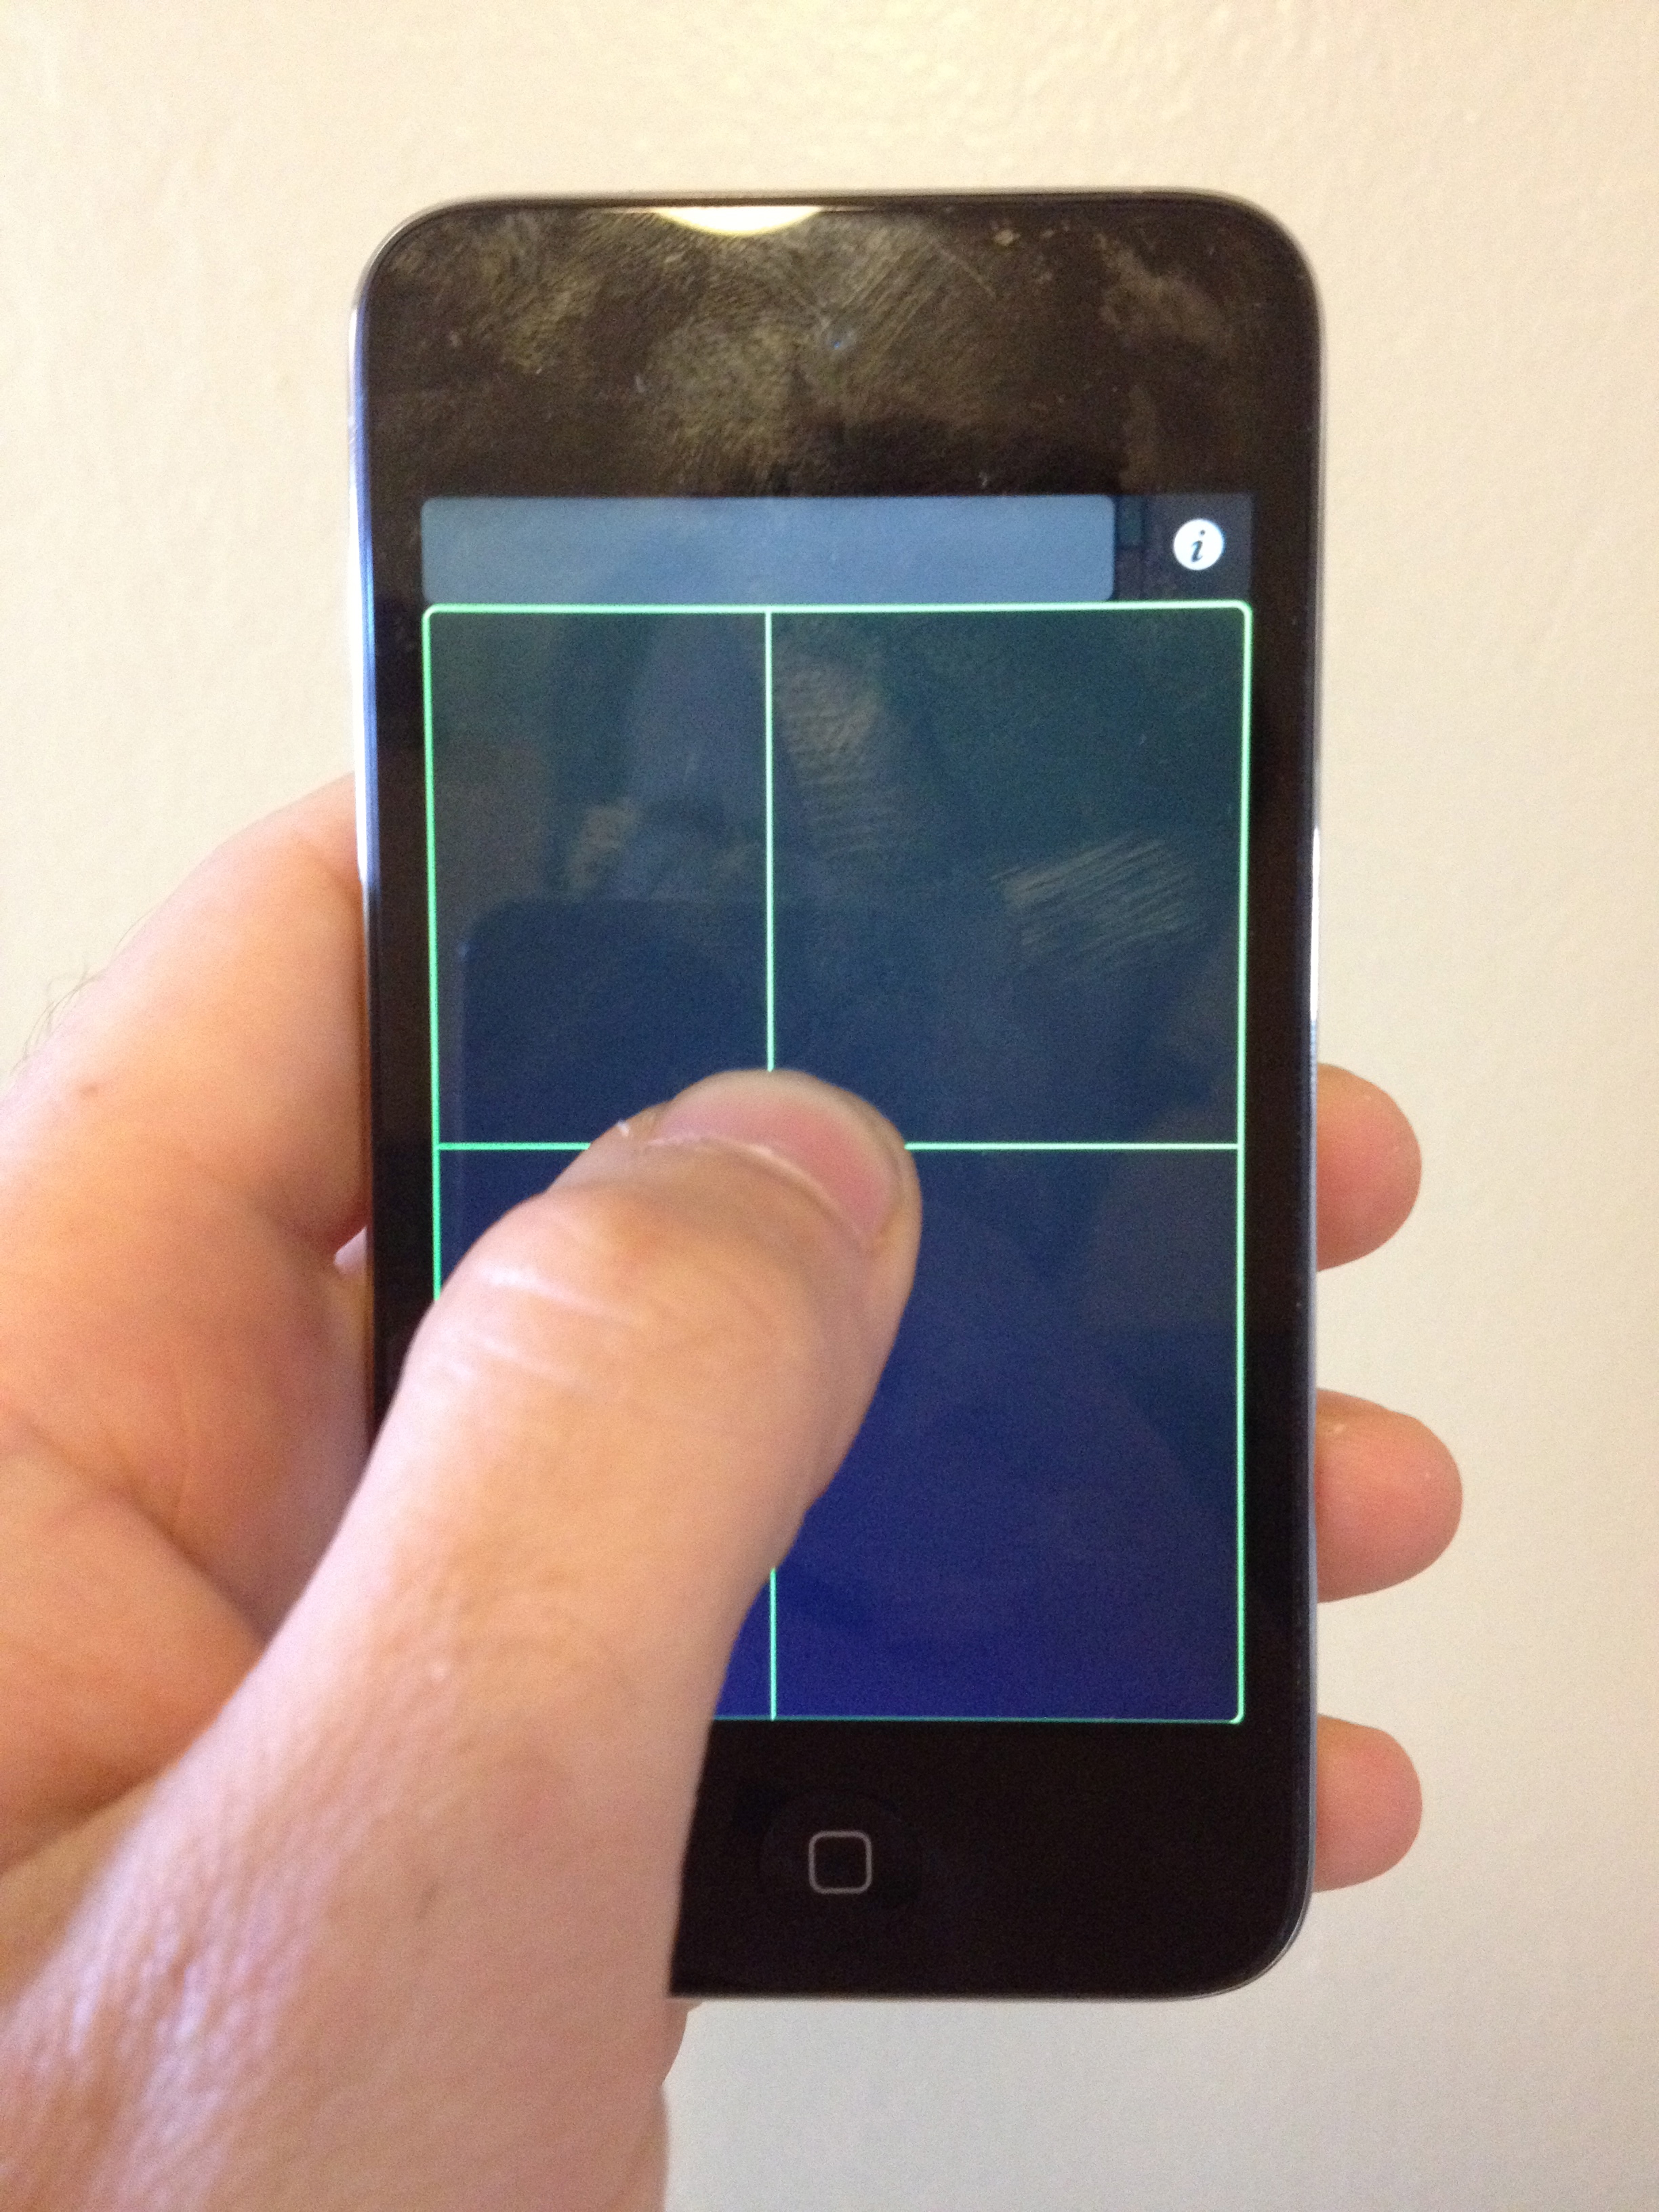
\includegraphics[width=\columnwidth]{iphone.jpg}
\caption{The instrument control on an iOS device. A new note is played when the finger touches or drags the surface.}
\label{iphone}
\end{figure}


\subsubsection{The Interaction}

The musical interaction is designed for two players.  Each plays their own instrument with their own iPhone controller, and each instrument has a slightly different tone (a sawtooth wave for one and a square wave for the other.)  There is a shared public display where the players, as well as any bystanders, can see both players' actions.  The display appears as a single large rectangle mirroring the touch area on the iPhone controller.  Notes played on either instrument appear as colored circles in the rectangle with a different color for each player (see figure~\ref{screenshot-processing} a).

\begin{figure}[tb]
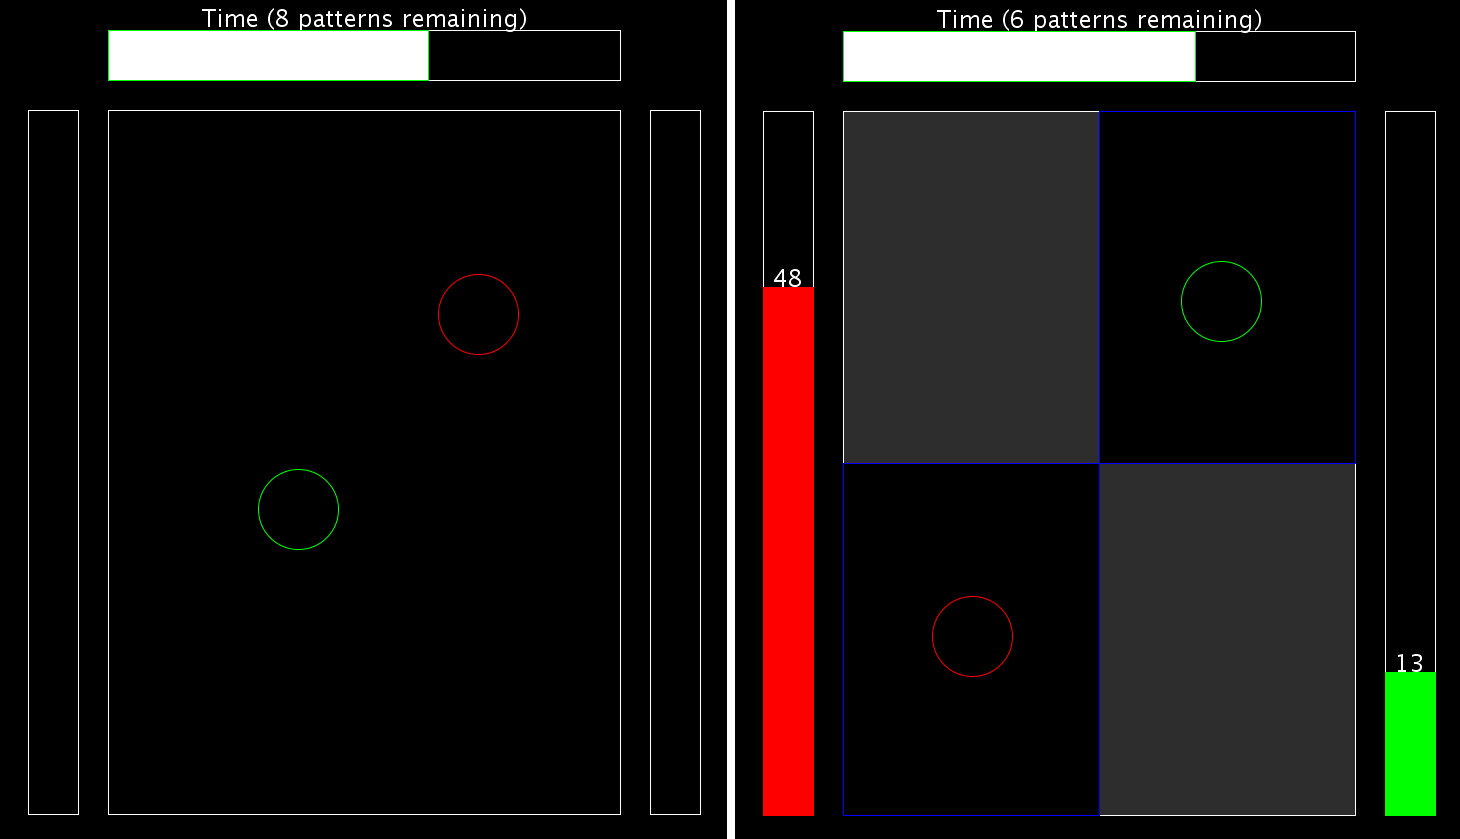
\includegraphics[width=\columnwidth]{screenshot-processing.png}
\caption{On the left, the general public shared screen. Player 1's position on the iOS device is reproduced here with a red circle, whereas the green circle correspond to player 2. On the right, adding structure to the interaction: players are encouraged to play in the black zones with a blue border. The bars on either side of the screen represent the number of notes left for each player in the current pattern.}
\label{struct}
\end{figure}

\subsubsection{Playing a Duet}

When users play a duet there is a background musical accompaniment of chords and a drum pattern.  The duet consists of 8 ``patterns'' of four measures each.  At a tempo of 100 beats per minutes a duet lasts one minute and twenty seconds.  A bar at the top of the display shows time progressing through each pattern, as well as the number of patterns left in the song.  

The notes that the instruments can play are constrained to a scale which sounds good with the chords of the duet.  Also the timing of notes are constrained to fall on 16th note intervals of the accompaniment's rhythm.  As a result the music performed will always sounds musically consistent.

\subsubsection{Adding Constraints to Create Structure}

The instrument can be thought of as enabling three basic musical dimensions: note \emph{pitch} (controlled by vertical location), note \emph{timbre} (horizontal location), and the \emph{density} of notes (a function of how frequently notes are played.)  We create structure by directing the players into different areas of this musical space at different times. During structured duets blue squares appear on the display as seen in Figure~\ref{screenshot-processing} b.  The players are instructed to play within these squares, and if they play outside of them their sounds becomes distorted. The boundaries of the structure squares change for each 4-bar “pattern” in the music. This serves to constrain the first two musical dimensions.

We control the third dimension, note density, by constraining the number of notes that a player can play during each pattern. Colored bars on either side of the screen indicate the number of notes left to each player for the current pattern.


\subsubsection{Implementation}

The instrument is controlled with a custom layout for the TouchOSC iOS app which sends Open Sound Control (OSC) messages over UDP to a computer.  On the computer a program written in ChucK performs the sound synthesis and sequencing as well as the logic for the structural constraints. The display is created by a Processing program on the same computer.



\subsection{The Experiment}
We performed a between subjects experiment.  Participants were grouped into pairs, and pairs were assigned to either the control or experimental condition.  We had eight pairs of participants divided into the two conditions. All participants were university students.

For each pair of participants the experiment proceeded as follows: The instrument was briefly demonstrated. Then participants had up to two minutes to learn the instrument by playing freely with no accompanying music.  Both participants learned their instrument simultaneously and could hear each other and see each other's actions on the display.  Following learning the instrument, the first duet was performed.  For the control coup the first duet was unstructured, and for the experimental group it was structured.
 
Following the first duet there was a brief pause.  During this pause the control group was given verbal suggestions for ways to structure their interactions.  The suggestions were equivalent to what the experimental group might infer from the constraints of the structured interaction.

Participants then performed a second duet together.  The musical accompaniment for the second duet was the same as for the first.  In the second duet both the control and experimental groups were given the unstructured interaction. The experiment is represented on figure~\cite{experiment}.

This design allows as to compare the duets between and within groups.  Given our hypotheses, we expected to find that in the first duet the experimental group was more enjoyable, due to the context provided by the structure. We also expected the the experimental group would create better music than the control group. We expected that within the experimental group the second duet would be less enjoyable, due to the loss of context when the structure was removed.  

We also expected that in the second duet the experimental group would perform musically as well or better than the control group, due to inferring principles of musical interaction from the structured interaction.

\begin{figure}[tb]
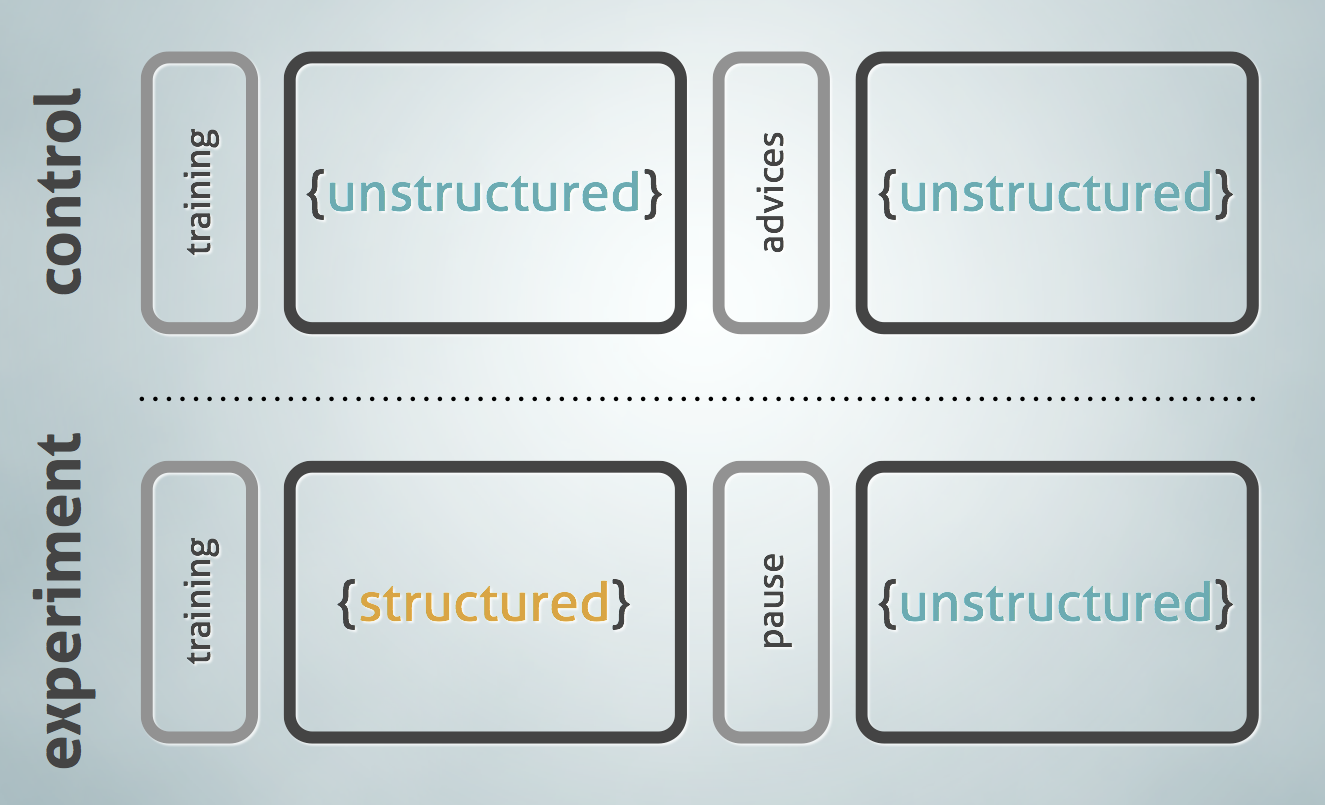
\includegraphics[width=\columnwidth]{exp.png}
\caption{The experiment. The control group 1) has a short period of training, 2) plays a duet without structure, 3) is given verbal instructions, 4) plays a second duet without structure. The experimental group 1) has a short period of training, 2) plays a duet with structure, 3) has a short pause, 4) plays a second duet without structure.}
\label{experiment}
\end{figure}


\section{RESULTS}

\subsection{From the Survey}

After the experiment, the participants completed a survey. For each duet, we asked them to evaluate on a Likert scale (from 1 to 7) the following metrics:
\begin{itemize}
\item their confidence,
\item their enjoyment,
\item how much they took the other player's actions into account,
\item how much they thought the other player took their actions into account,
\item how good they thought the resulting music was.
\end{itemize}
For each group, we compared the scores assigned to each duet. We found that participants in the experimental group enjoyed the second duet more than the first ($t(14) = 2.89$, $p = 0.006$), took their partner into account more in the second duet ($t(14) = 2.09$, $p = 0.028$), and thought that the music was better in the second duet ($t(14) = 3.47$, $p = 0.002$).

Furthermore, we calculated the increase of these metrics between duet 1 and duet 2, and compared the difference between the control and the experimental group. We find two results:
\begin{itemize}
\item the increase in the enjoyment from duet 1 to duet 2 is greater in the experimental group than in the control group ($t(14) = 1.85$, $p = 0.043$),
\item the increase in the perceived music quality from duet 1 to duet 2 is greater in the experimental group ($t(14) = 2.17, p = 0.024$).
\end{itemize}
These results correlate with and confirm the previous results by removing any bias due to different means between the groups: for the experimental group, the experience was significantly better in the second duet than in the first.


\subsection{Crowdsourcing the Evaluation of the Musical Quality}

Musical quality is an inherently subjective judgement, and thus difficult to objectively assess.  However by soliciting judgements from a large number of people we can hope to average out personal preferences and perhaps converge on some measure of quality.  We created a web site which asked visitors to compare recordings of two duets and indicate which was better.  We advertised for evaluators by posting on Facebook and various email lists, and within 48 hours we gathered 474 evaluations, coming from 114 different IP addresses. By using the Elo rating system, which computes the relative scores of a group of ordered pairs, we were able to rank duets in terms of musical quality.

We performed separate ratings of the recordings of all the first duets (for both groups), and all the second duets (also both groups.)  Table~\ref{musicmash-results} shows the ranking among the songs in duet 1. These scores had a standard deviation of $44.05$ and a mean of $1500$.  The music produced by group 3 is almost two standard deviations below the mean ($\Delta = 86$), and thus we considered this data point an outlier, and removed it from our dataset.

Figure~\ref{survey-results} shows the average Elo score of the music performed with structure, and the music performed without structure. The average score of the music performed with structure is significantly greater than the score of the music performed without structure ($t(6) = 3.55$, $p = 0.006$). In other words, people preferred music played with structure to music played without structure.  We did not find any trend in the ranking of the second duets.

\begin{table}[tb]
\begin{center}
\begin{tabular}{l r}
Group & Elo score \\
\hline
Experimental & 1562 \\
Experimental & 1534 \\
Experimental & 1522 \\
Control & 1509 \\
Control & 1490 \\
Control & 1489 \\
Control & 1480 \\
Experimental & 1414 \\
\end{tabular}
\caption{Ranking of recordings made of the first duets in terms of musical quality. The experimental group performed music with structure; the control group performed music without structure.} 
\label{musicmash-results}
\end{center}
\end{table}

\begin{figure}[tb]
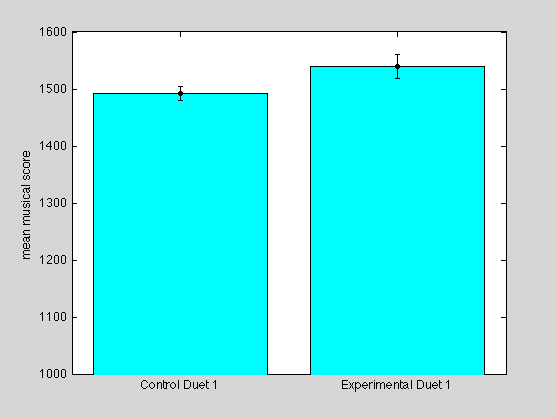
\includegraphics[width=\columnwidth]{music-scores-bar-graph.png}
\caption{Musical quality of the first duets for the control (unstructured) and experimental (structured) conditions.} 
\label{survey-results}
\end{figure}

% edited thru here... LUke

\subsection{Analyzing Notes}

We recorded all note data during the duet performances, and calculated three metrics to quantify the musical parameter of note density. The percent of notes played tells us how many total notes were played. The percent of time with no notes tells us how often neither player was playing, \emph{i.e.} how much space the players left. And the percent of notes with only one player tells is the proportion of time when a note was played that only one player was playing at that time, which tells us how much the players took turns. Each of these metric has an obvious trend when we plot from the duets from the Control group to those of the Experiment group, as we can see on figure~\ref{note-stats}. The first increased, while the second two decrease. A significant difference between these results appears when we compare the second duet of the control with that of the experiment. The control group played fewer notes ($p = 0.048$) and had higher proportion of single notes, \emph{i.e.} they exhibited more turn taking ($p = 0.035$). In some sense this suggests that the control group played better music during the second duet. 

\begin{figure}[tb]
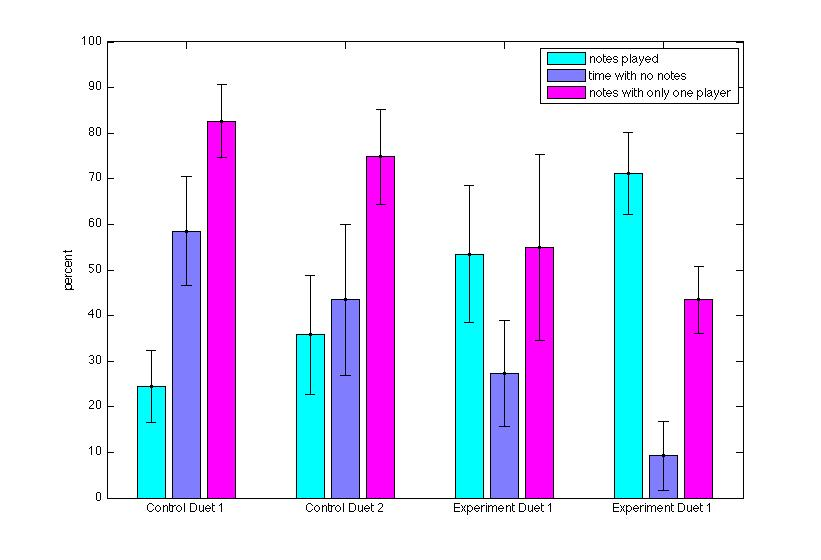
\includegraphics[width=\columnwidth]{note_analysis_new.jpg}
\caption{Note repartition in the different duets.} 
\label{note-stats}
\end{figure}




\section{DISCUSSION}

Our goal was to better understand musical interactions for novices by dividing the interface into instrument and interactions, and then to investigate the effect of adding structure to the interaction.  Our crowd-sourced evaluation of the musical results showed that adding structure clearly leads to better music.  However it is less clear whether adding structure led to a better experience for the user.  

From the survey we found that users who played two unstructured duets had no significant change in their experience between duets, while those who had a structured interaction in the first duet had a better experience in the second unstructured duet. We can interpret this in either of two conflicting ways.

The first is that the second duet was better because the previous structured interaction increased the users' confidence in performing duets with the instrument. From the interviews a few people (3 out of 16) explicitly reported that they liked the structural constraints because like a game, they provided goals, but none reported that they thought of the constraints during the second duet. Following those ideas, 
further studies could consist in:
\begin{itemize}
\item exploring if the structure in the first duet actually taught musical principles (consciously or subconsciously) to the novices,
\item analyzing if structured interaction could be used as an efficient \textit{training} for better enjoyment during an actual performance. Indeed, the level of enjoyment for the first duet is similar in both groups, but the second duet was significantly better enjoyed in the experimental group. Instead of seeing the first duets as \textit{performances}, we could see them as \textit{trainings}. In that case, it would be interesting to study if a \textit{training} period with structure leads to better experience for a subsequent \textit{performance}.
\end{itemize}

The second interpretation of the increase in enjoyment from structured to unstructured interaction, is that the structured interactions were not as enjoyable as unstructured.  A number of participants (4 out of 16) explicitly reported that it was difficult to quickly understand all the visual feedback being provided during structured interactions.  Though we attempted to design a simple instrument with simple interaction constraints, the net effect was to create a complicated interaction.

Despite any differences between the interaction types, almost all participants reported enjoying the experience, and being pleased with being able to easily make relatively good-sounding music.




\section{CONCLUSION}

In this study, we investigated the effects of adding structural guidelines to musical interactions for novices. The instrument we designed allowed novices to play the music with simple interactions, which could be constrained by adding structure to the three parameters (pitch, timber, and note density). People were divided into two groups: a control group were pairs of people had to play a series of two duets without structure, and an experimental group where the first duet had structured interaction and the second was unstructured. The analysis of the music quality in the pieces produced in the different groups let us find that structure significantly improved the quality of the music. The results of the post experiment survey showed that the experimental group had a better experience during the second unstructured duet.




\section{ACKNOWLEDGMENTS}

The authors would like to acknowledge Professor Scott Klemmer, Chinmay Kulkarni, and the participants of our experiments for their time and input.

%%%	You can use bibtex if you like, but I've hardwired in these 
%%%	references to avoid sending you a separate .bib file.
\begin{thebibliography}{9}

\bibitem{smule} Wang, G., G. Essl, J. Smith, S. Salazar, P. Cook, R. Hamilton, R. Fiebrink, J. Berger, D. Zhu, M. Ljungstrom, A. Berry, J. Wu, T. Kirk, E. Berger, J. Segal. Smule = Sonic Media: An Intersection of the Mobile, Musical, and Social.
In {\em Proceedings of the International Computer Music Conference.}
Montreal, 2009.

\bibitem{smule-2} Wang, G. Designing Smule's iPhone Ocarina.
In {\em Proceedings of the International Conference on New Interfaces for Musical Expression.}
Pittsburgh, 2009.


\bibitem{metris} Havryliv, M., Narushima, T., Metris: a Game Environment for Music Performance.

\bibitem{survey} Blaine, T., Fels, S. Collaborative Musical Experiences for Novices.
Journal of New Music Research, 32:4, 411-428, 2003.
In {\em Proceedings of Computer Music Modeling and Retrieval.}
2005.

\end{thebibliography}

\end{document}
